\section{Objetivos}

Entre otros, el principal objetivo de MIEX es analizar sint�ctica y
sem�nticamente colecciones de peque�os documentos escritos en ingl�s.

Aprovechando las capacidades del analizador (Stanford Parser) se realizan dos
tipos de an�lisis. En primer lugar un an�lisis sint�ctico de la oraci�n y
posteriormente un an�lisis sem�ntico con el fin de obtener las relaciones entre
las palabras de cada una de las oraciones. La mejor manera de ilustrar estos
conceptos es utilizando un peque�o ejemplo, por lo que veamos que an�lisis
produce el analizador para la siguiente oraci�n.

\begin{center}
\textit{The Debian Project is an association of individuals.}
\end{center}

Si bien la representaci�n gr�fica del an�lisis sint�ctico es m�s habitual
hacerla de la forma cl�sica (subrayando cada elemento de la oraci�n), la manera
m�s visual y l�gica es utilizar un �rbol (figura \ref{fig:arbol-sintactico}).

\begin{figure}[h]
\centering
\Tree[.ROOT [.S [.NP [.DT The ] [.NNP Debian ] [.NNP Project ] ] [.VP [.VBZ is
] [.NP [.NP [.DT an ] [.NN association ] ] [.PP [.IN of ] [.NP [.NNS individuals
 ] ] ] ] ] ] ]
\caption{Ejemplo de representaci�n en forma de �rbol de un an�lisis sint�ctico}
\label{fig:arbol-sintactico}
\end{figure} 
 
Se puede apreciar como se asignan etiquetas a nivel de palabra, a nivel de
grupo frasal y a nivel clausal, tal y como se hace habitualmente en cualquier
an�lisis sint�ctico. Si desea conocer el significado de cada etiqueta no tiene
m�s que echar un vistazo a los ap�ndices \ref{cha:penntags} y
\ref{cha:gramrelations}. Aprovecharemos tambi�n que el analizador calcula las
dependencias entre algunas palabras de la oraci�n
(figura \ref{fig:relaciones-palabras}).

\begin{figure}[h]
\centering
\begin{Verbatim}[frame=single,framesep=10pt,fontsize=\relsize{-1}]
det(Project-3, The-1)
nn(Project-3, Debian-2)
nsubj(association-6, Project-3)
cop(association-6, is-4)
det(association-6, an-5)
prep_of(association-6, individuals-8)
\end{Verbatim}
\caption{Ejemplo de representaci�n de relaciones entre palabras de una oraci�n}
\label{fig:relaciones-palabras}
\end{figure}

Tanto el an�lisis a nivel de palabra (y obviamente a nivel de grupo), como las
relaciones entre las palabras, ser� la informaci�n que nos va a interesar
guardar m�s adelante.

Aunque en el siguiente cap�tulo se explica con m�s detalle cada uno de los
pasos en los que se divide la ejecuci�n, una visi�n global de los objetivos que
cumple MIEX es la siguiente:

\begin{itemize}
	\item Comprobaci�n de integridad y an�lisis de documentos XML.
	\item Uso del Stanford Parser para extraer los an�lisis
sint�cticos de las oraciones as� como las relaciones entre las palabras.
	\item An�lisis y limpieza de la informaci�n recabada.
	\item Almacenamiento en un medio flexible para posteriormente realizar
consultas a medida.
\end{itemize}

\begin{figure}[h]
\begin{center}
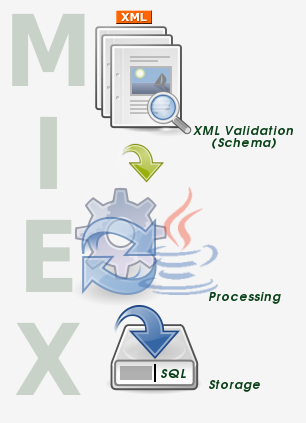
\includegraphics[bb=0 0 148 240]{images/miex.png}
\end{center}
\caption{Diagrama simplificado de funcionamiento}
\end{figure} 
